\documentclass[14pt]{extbook}
\usepackage{multicol, enumerate, enumitem, hyperref, color, soul, setspace, parskip, fancyhdr} %General Packages
\usepackage{amssymb, amsthm, amsmath, latexsym, units, mathtools} %Math Packages
\everymath{\displaystyle} %All math in Display Style
% Packages with additional options
\usepackage[headsep=0.5cm,headheight=12pt, left=1 in,right= 1 in,top= 1 in,bottom= 1 in]{geometry}
\usepackage[usenames,dvipsnames]{xcolor}
\usepackage{dashrule}  % Package to use the command below to create lines between items
\newcommand{\litem}[1]{\item#1\hspace*{-1cm}\rule{\textwidth}{0.4pt}}
\pagestyle{fancy}
\lhead{Makeup Progress Quiz 3}
\chead{}
\rhead{Version ALL}
\lfoot{1648-1753}
\cfoot{}
\rfoot{Summer C 2021}
\begin{document}

\begin{enumerate}
\litem{
Determine the domain of the function below.\[ f(x) = \frac{4}{15x^{2} -5 x -20} \]\begin{enumerate}[label=\Alph*.]
\item \( \text{All Real numbers.} \)
\item \( \text{All Real numbers except } x = a, \text{ where } a \in [-5, 0] \)
\item \( \text{All Real numbers except } x = a, \text{ where } a \in [-27, -22] \)
\item \( \text{All Real numbers except } x = a \text{ and } x = b, \text{ where } a \in [-5, 0] \text{ and } b \in [-0.67, 5.33] \)
\item \( \text{All Real numbers except } x = a \text{ and } x = b, \text{ where } a \in [-27, -22] \text{ and } b \in [10, 15] \)

\end{enumerate} }
\litem{
Solve the rational equation below. Then, choose the interval(s) that the solution(s) belongs to.\[ \frac{12}{-54x + 12} + 1 = \frac{12}{-54x + 12} \]\begin{enumerate}[label=\Alph*.]
\item \( x \in [-0.78,2.22] \)
\item \( x_1 \in [-0.9, 0.2] \text{ and } x_2 \in [0.22,3.22] \)
\item \( \text{All solutions lead to invalid or complex values in the equation.} \)
\item \( x_1 \in [-0.2, 0.8] \text{ and } x_2 \in [0.22,3.22] \)
\item \( x \in [-0.9,0.2] \)

\end{enumerate} }
\litem{
Choose the equation of the function graphed below.
\begin{center}
    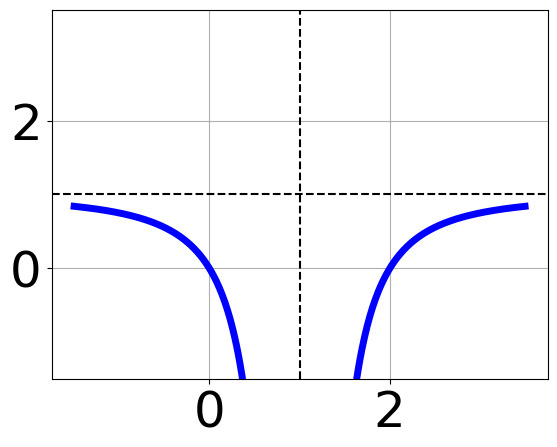
\includegraphics[width=0.5\textwidth]{../Figures/rationalGraphToEquationCopyA.png}
\end{center}
\begin{enumerate}[label=\Alph*.]
\item \( f(x) = \frac{1}{x - 1} + 1 \)
\item \( f(x) = \frac{-1}{x + 1} + 1 \)
\item \( f(x) = \frac{-1}{(x + 1)^2} + 1 \)
\item \( f(x) = \frac{1}{(x - 1)^2} + 1 \)
\item \( \text{None of the above} \)

\end{enumerate} }
\litem{
Choose the graph of the equation below.\[ f(x) = \frac{-1}{x - 3} + 3 \]\begin{enumerate}[label=\Alph*.]
\begin{multicols}{2}\item 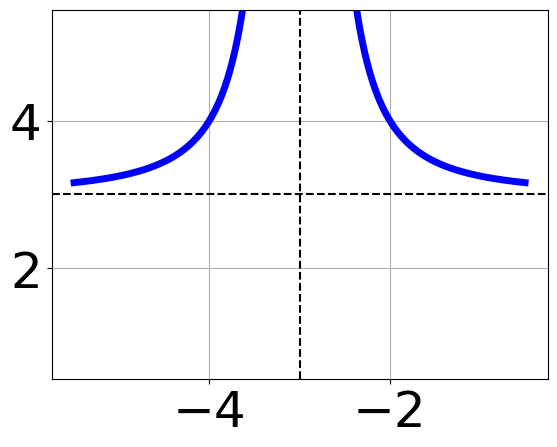
\includegraphics[width = 0.3\textwidth]{../Figures/rationalEquationToGraphCopyAA.png}\item 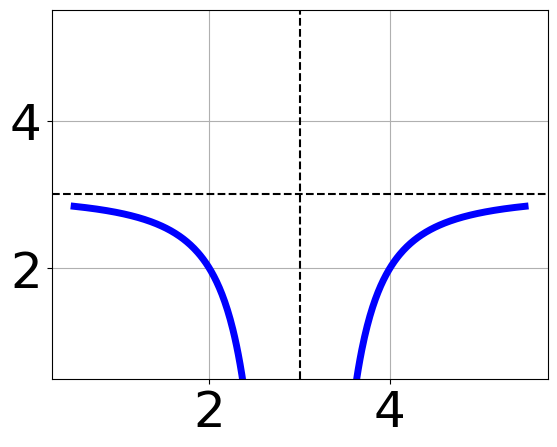
\includegraphics[width = 0.3\textwidth]{../Figures/rationalEquationToGraphCopyBA.png}\item 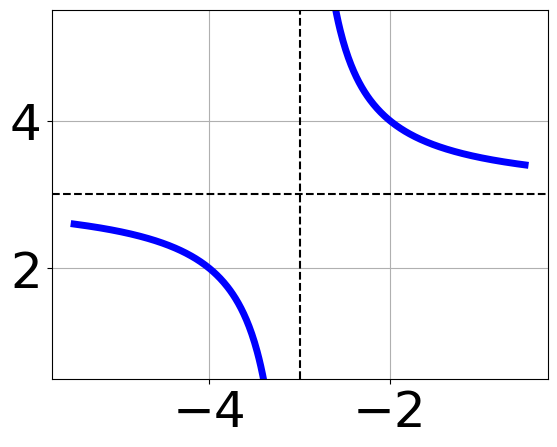
\includegraphics[width = 0.3\textwidth]{../Figures/rationalEquationToGraphCopyCA.png}\item 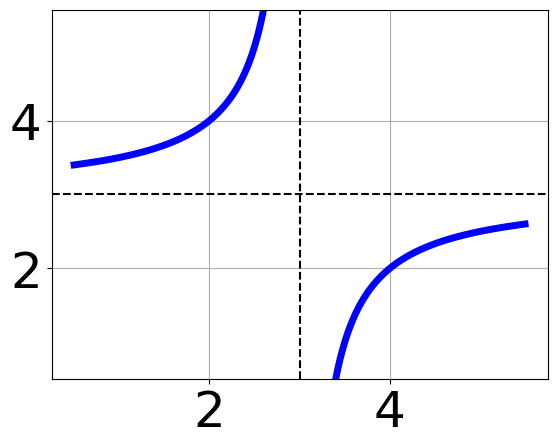
\includegraphics[width = 0.3\textwidth]{../Figures/rationalEquationToGraphCopyDA.png}\end{multicols}\item None of the above.
\end{enumerate} }
\litem{
Determine the domain of the function below.\[ f(x) = \frac{6}{18x^{2} -48 x + 30} \]\begin{enumerate}[label=\Alph*.]
\item \( \text{All Real numbers except } x = a \text{ and } x = b, \text{ where } a \in [0.08, 1.26] \text{ and } b \in [1.34, 2.24] \)
\item \( \text{All Real numbers.} \)
\item \( \text{All Real numbers except } x = a, \text{ where } a \in [14.2, 15.35] \)
\item \( \text{All Real numbers except } x = a, \text{ where } a \in [0.08, 1.26] \)
\item \( \text{All Real numbers except } x = a \text{ and } x = b, \text{ where } a \in [14.2, 15.35] \text{ and } b \in [35.49, 36.48] \)

\end{enumerate} }
\litem{
Solve the rational equation below. Then, choose the interval(s) that the solution(s) belongs to.\[ \frac{-3}{9x + 7} + 8 = \frac{-8}{-81x -63} \]\begin{enumerate}[label=\Alph*.]
\item \( x \in [0.7,0.98] \)
\item \( x \in [-1.72,1.28] \)
\item \( x_1 \in [-0.73, -0.57] \text{ and } x_2 \in [0.2,1.3] \)
\item \( \text{All solutions lead to invalid or complex values in the equation.} \)
\item \( x_1 \in [-1.11, -0.79] \text{ and } x_2 \in [-1.2,-0.2] \)

\end{enumerate} }
\litem{
Choose the graph of the equation below.\[ f(x) = \frac{-1}{(x + 3)^2} + 2 \]\begin{enumerate}[label=\Alph*.]
\begin{multicols}{2}\item 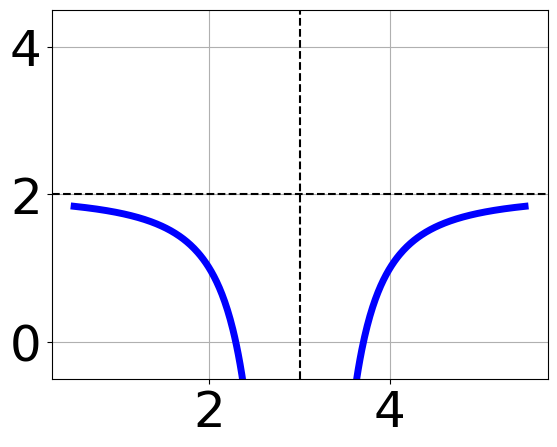
\includegraphics[width = 0.3\textwidth]{../Figures/rationalEquationToGraphAA.png}\item 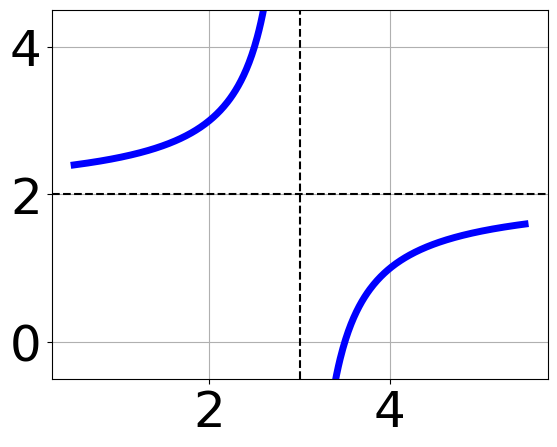
\includegraphics[width = 0.3\textwidth]{../Figures/rationalEquationToGraphBA.png}\item 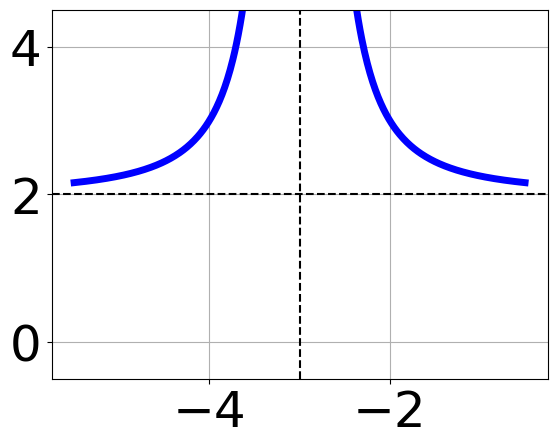
\includegraphics[width = 0.3\textwidth]{../Figures/rationalEquationToGraphCA.png}\item 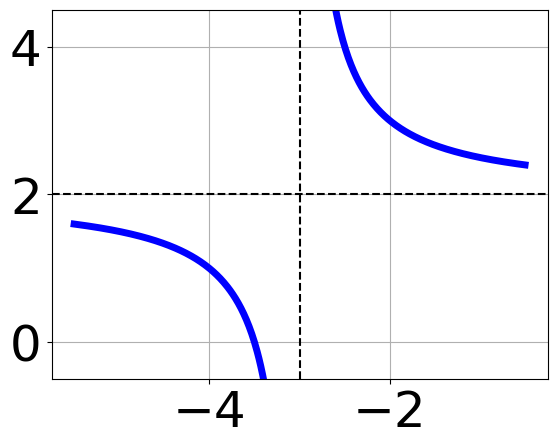
\includegraphics[width = 0.3\textwidth]{../Figures/rationalEquationToGraphDA.png}\end{multicols}\item None of the above.
\end{enumerate} }
\litem{
Choose the equation of the function graphed below.
\begin{center}
    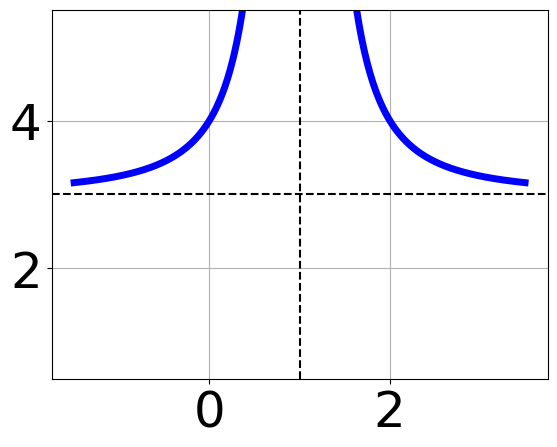
\includegraphics[width=0.5\textwidth]{../Figures/rationalGraphToEquationA.png}
\end{center}
\begin{enumerate}[label=\Alph*.]
\item \( f(x) = \frac{-1}{x + 1} + 3 \)
\item \( f(x) = \frac{-1}{(x + 1)^2} + 3 \)
\item \( f(x) = \frac{1}{(x - 1)^2} + 3 \)
\item \( f(x) = \frac{1}{x - 1} + 3 \)
\item \( \text{None of the above} \)

\end{enumerate} }
\litem{
Solve the rational equation below. Then, choose the interval(s) that the solution(s) belongs to.\[ \frac{-4x}{-6x -6} + \frac{-2x^{2}}{-12x^{2} +12 x + 24} = \frac{-3}{2x -4} \]\begin{enumerate}[label=\Alph*.]
\item \( x_1 \in [-1.52, -0.93] \text{ and } x_2 \in [0,4] \)
\item \( \text{All solutions lead to invalid or complex values in the equation.} \)
\item \( x \in [-1.52,-0.93] \)
\item \( x \in [1.74,3.27] \)
\item \( x_1 \in [1.03, 1.6] \text{ and } x_2 \in [-4.89,-0.89] \)

\end{enumerate} }
\litem{
Solve the rational equation below. Then, choose the interval(s) that the solution(s) belongs to.\[ \frac{3x}{5x -2} + \frac{-2x^{2}}{15x^{2} -26 x + 8} = \frac{-4}{3x -4} \]\begin{enumerate}[label=\Alph*.]
\item \( x \in [-3.37,0.31] \)
\item \( x \in [0.82,2.75] \)
\item \( x_1 \in [-0.86, 0.67] \text{ and } x_2 \in [0.4,2.4] \)
\item \( x_1 \in [-0.86, 0.67] \text{ and } x_2 \in [-4.78,0.22] \)
\item \( \text{All solutions lead to invalid or complex values in the equation.} \)

\end{enumerate} }
\litem{
Determine the domain of the function below.\[ f(x) = \frac{6}{24x^{2} +6 x -9} \]\begin{enumerate}[label=\Alph*.]
\item \( \text{All Real numbers except } x = a \text{ and } x = b, \text{ where } a \in [-2, 0.2] \text{ and } b \in [-0.3, 2.5] \)
\item \( \text{All Real numbers except } x = a \text{ and } x = b, \text{ where } a \in [-12.4, -11.6] \text{ and } b \in [17.4, 19.7] \)
\item \( \text{All Real numbers.} \)
\item \( \text{All Real numbers except } x = a, \text{ where } a \in [-2, 0.2] \)
\item \( \text{All Real numbers except } x = a, \text{ where } a \in [-12.4, -11.6] \)

\end{enumerate} }
\litem{
Solve the rational equation below. Then, choose the interval(s) that the solution(s) belongs to.\[ \frac{5}{-3x -7} + 5 = \frac{6}{9x + 21} \]\begin{enumerate}[label=\Alph*.]
\item \( x \in [2.63,2.81] \)
\item \( x_1 \in [-2.06, -1.55] \text{ and } x_2 \in [1.8,3.8] \)
\item \( x \in [-1.87,-0.87] \)
\item \( x_1 \in [-2.46, -1.99] \text{ and } x_2 \in [-1.87,0.13] \)
\item \( \text{All solutions lead to invalid or complex values in the equation.} \)

\end{enumerate} }
\litem{
Choose the equation of the function graphed below.
\begin{center}
    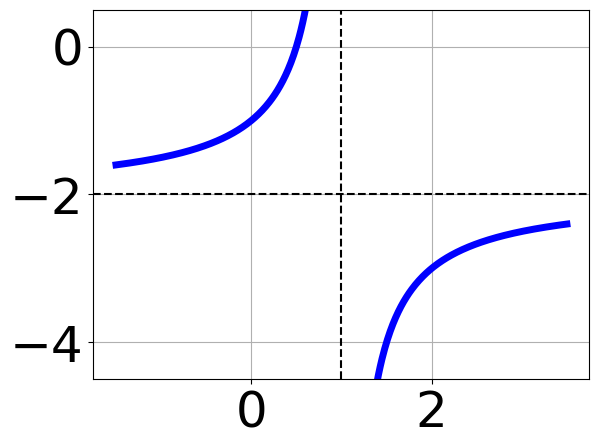
\includegraphics[width=0.5\textwidth]{../Figures/rationalGraphToEquationCopyB.png}
\end{center}
\begin{enumerate}[label=\Alph*.]
\item \( f(x) = \frac{1}{(x - 1)^2} + 4 \)
\item \( f(x) = \frac{1}{x - 1} + 4 \)
\item \( f(x) = \frac{-1}{(x + 1)^2} + 4 \)
\item \( f(x) = \frac{-1}{x + 1} + 4 \)
\item \( \text{None of the above} \)

\end{enumerate} }
\litem{
Choose the graph of the equation below.\[ f(x) = \frac{1}{x + 3} - 1 \]\begin{enumerate}[label=\Alph*.]
\begin{multicols}{2}\item 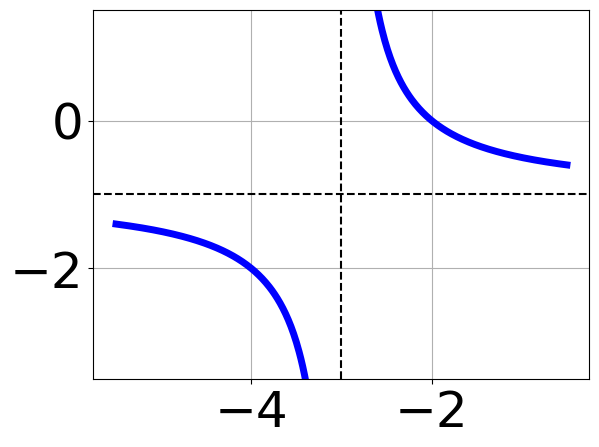
\includegraphics[width = 0.3\textwidth]{../Figures/rationalEquationToGraphCopyAB.png}\item 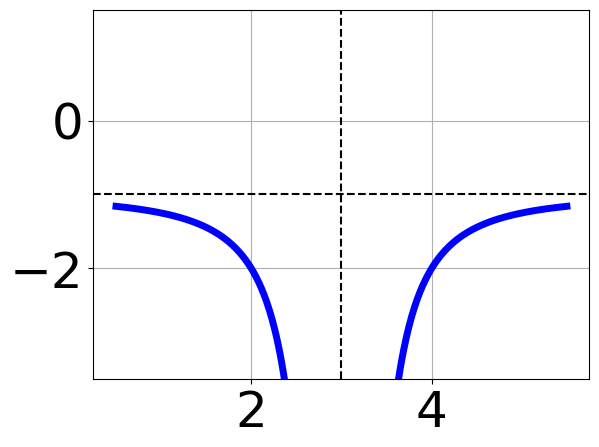
\includegraphics[width = 0.3\textwidth]{../Figures/rationalEquationToGraphCopyBB.png}\item 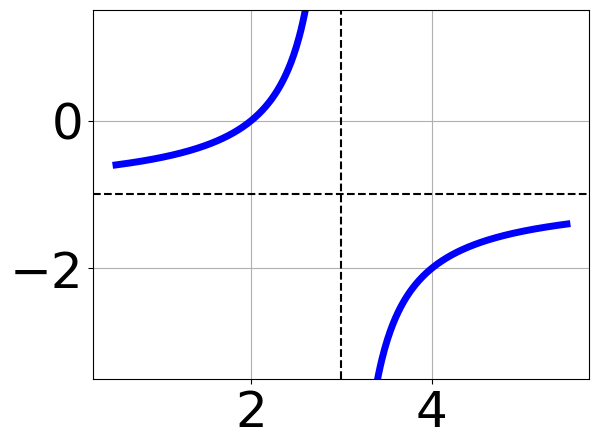
\includegraphics[width = 0.3\textwidth]{../Figures/rationalEquationToGraphCopyCB.png}\item 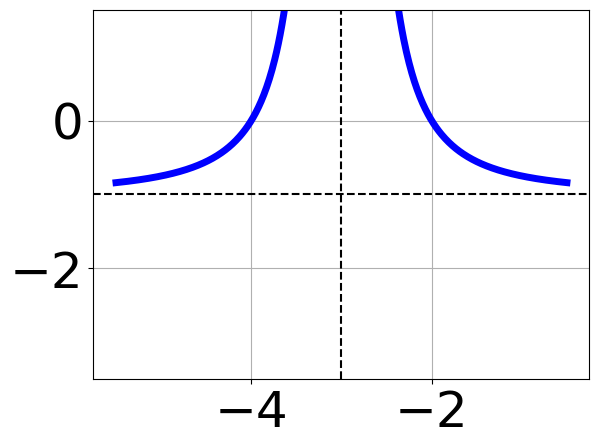
\includegraphics[width = 0.3\textwidth]{../Figures/rationalEquationToGraphCopyDB.png}\end{multicols}\item None of the above.
\end{enumerate} }
\litem{
Determine the domain of the function below.\[ f(x) = \frac{3}{12x^{2} -36 x + 24} \]\begin{enumerate}[label=\Alph*.]
\item \( \text{All Real numbers except } x = a \text{ and } x = b, \text{ where } a \in [14.7, 16.9] \text{ and } b \in [17, 18.2] \)
\item \( \text{All Real numbers except } x = a, \text{ where } a \in [-1.1, 1.7] \)
\item \( \text{All Real numbers except } x = a, \text{ where } a \in [14.7, 16.9] \)
\item \( \text{All Real numbers except } x = a \text{ and } x = b, \text{ where } a \in [-1.1, 1.7] \text{ and } b \in [1.7, 2.9] \)
\item \( \text{All Real numbers.} \)

\end{enumerate} }
\litem{
Solve the rational equation below. Then, choose the interval(s) that the solution(s) belongs to.\[ \frac{3}{5x + 4} + -7 = \frac{2}{-20x -16} \]\begin{enumerate}[label=\Alph*.]
\item \( x \in [0.87,0.94] \)
\item \( x \in [-1.7,1.3] \)
\item \( \text{All solutions lead to invalid or complex values in the equation.} \)
\item \( x_1 \in [-0.7, -0.69] \text{ and } x_2 \in [0.9,5.9] \)
\item \( x_1 \in [-0.79, -0.72] \text{ and } x_2 \in [-0.7,0.3] \)

\end{enumerate} }
\litem{
Choose the graph of the equation below.\[ f(x) = \frac{-1}{x - 2} - 2 \]\begin{enumerate}[label=\Alph*.]
\begin{multicols}{2}\item 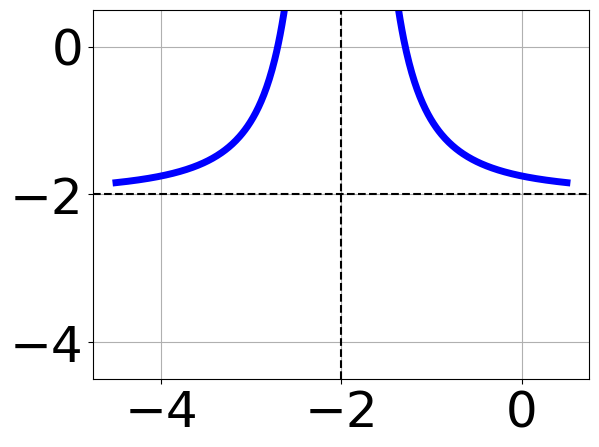
\includegraphics[width = 0.3\textwidth]{../Figures/rationalEquationToGraphAB.png}\item 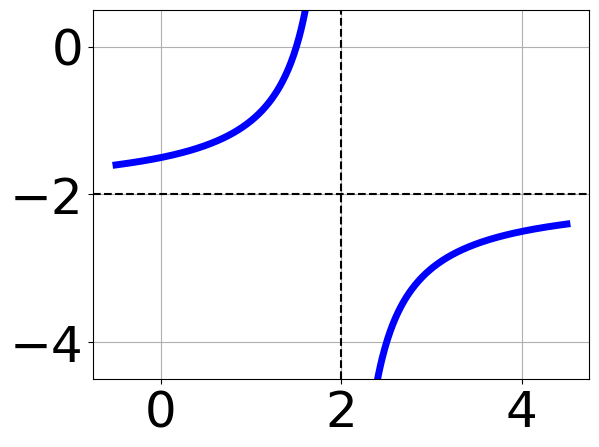
\includegraphics[width = 0.3\textwidth]{../Figures/rationalEquationToGraphBB.png}\item 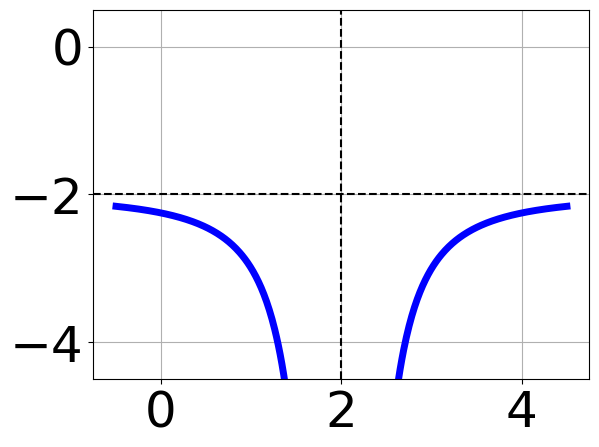
\includegraphics[width = 0.3\textwidth]{../Figures/rationalEquationToGraphCB.png}\item 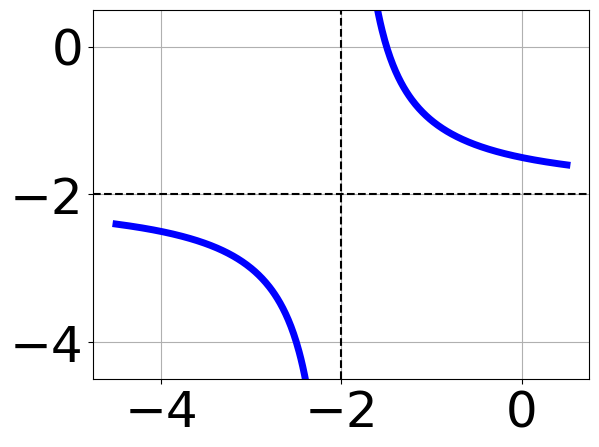
\includegraphics[width = 0.3\textwidth]{../Figures/rationalEquationToGraphDB.png}\end{multicols}\item None of the above.
\end{enumerate} }
\litem{
Choose the equation of the function graphed below.
\begin{center}
    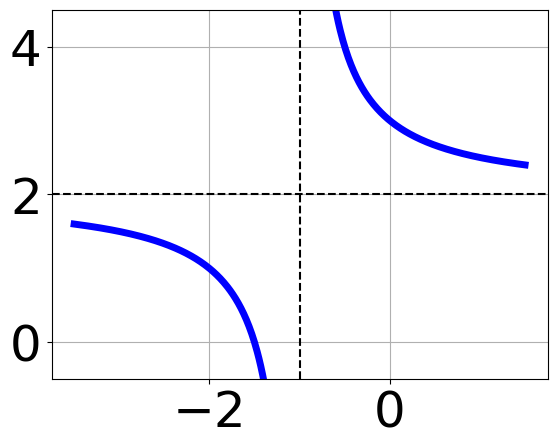
\includegraphics[width=0.5\textwidth]{../Figures/rationalGraphToEquationB.png}
\end{center}
\begin{enumerate}[label=\Alph*.]
\item \( f(x) = \frac{-1}{(x - 1)^2} + 2 \)
\item \( f(x) = \frac{-1}{x - 1} + 2 \)
\item \( f(x) = \frac{1}{x + 1} + 2 \)
\item \( f(x) = \frac{1}{(x + 1)^2} + 2 \)
\item \( \text{None of the above} \)

\end{enumerate} }
\litem{
Solve the rational equation below. Then, choose the interval(s) that the solution(s) belongs to.\[ \frac{5x}{3x + 5} + \frac{-2x^{2}}{18x^{2} +39 x + 15} = \frac{-6}{6x + 3} \]\begin{enumerate}[label=\Alph*.]
\item \( x_1 \in [-2.39, -1.64] \text{ and } x_2 \in [-0.56,-0.38] \)
\item \( x \in [-2.39,-1.64] \)
\item \( x_1 \in [-1.48, -0.61] \text{ and } x_2 \in [-0.17,1.79] \)
\item \( \text{All solutions lead to invalid or complex values in the equation.} \)
\item \( x \in [-0.75,-0.03] \)

\end{enumerate} }
\litem{
Solve the rational equation below. Then, choose the interval(s) that the solution(s) belongs to.\[ \frac{-5x}{2x -6} + \frac{-6x^{2}}{14x^{2} -28 x -42} = \frac{2}{7x + 7} \]\begin{enumerate}[label=\Alph*.]
\item \( \text{All solutions lead to invalid or complex values in the equation.} \)
\item \( x_1 \in [0.16, 0.32] \text{ and } x_2 \in [2,6] \)
\item \( x \in [-1.05,-0.78] \)
\item \( x_1 \in [0.16, 0.32] \text{ and } x_2 \in [-6.2,2.8] \)
\item \( x \in [-1.23,-1.17] \)

\end{enumerate} }
\litem{
Determine the domain of the function below.\[ f(x) = \frac{6}{30x^{2} -7 x -15} \]\begin{enumerate}[label=\Alph*.]
\item \( \text{All Real numbers.} \)
\item \( \text{All Real numbers except } x = a \text{ and } x = b, \text{ where } a \in [-1.42, -0.37] \text{ and } b \in [0.6, 1.37] \)
\item \( \text{All Real numbers except } x = a, \text{ where } a \in [-1.42, -0.37] \)
\item \( \text{All Real numbers except } x = a \text{ and } x = b, \text{ where } a \in [-16.01, -14.82] \text{ and } b \in [29.58, 30.49] \)
\item \( \text{All Real numbers except } x = a, \text{ where } a \in [-16.01, -14.82] \)

\end{enumerate} }
\litem{
Solve the rational equation below. Then, choose the interval(s) that the solution(s) belongs to.\[ \frac{-63}{-35x + 14} + 1 = \frac{-63}{-35x + 14} \]\begin{enumerate}[label=\Alph*.]
\item \( x_1 \in [-0.3, 1] \text{ and } x_2 \in [-3.6,1.4] \)
\item \( x_1 \in [-0.8, 0] \text{ and } x_2 \in [-3.6,1.4] \)
\item \( \text{All solutions lead to invalid or complex values in the equation.} \)
\item \( x \in [0.4,1.4] \)
\item \( x \in [-0.8,0] \)

\end{enumerate} }
\litem{
Choose the equation of the function graphed below.
\begin{center}
    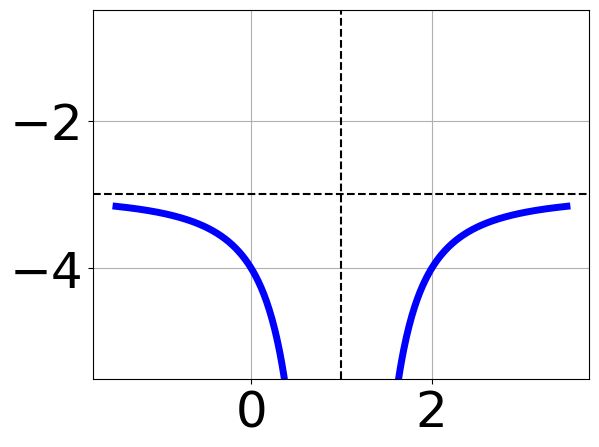
\includegraphics[width=0.5\textwidth]{../Figures/rationalGraphToEquationCopyC.png}
\end{center}
\begin{enumerate}[label=\Alph*.]
\item \( f(x) = \frac{-1}{x + 1} + 4 \)
\item \( f(x) = \frac{-1}{(x + 1)^2} + 4 \)
\item \( f(x) = \frac{1}{x - 1} + 4 \)
\item \( f(x) = \frac{1}{(x - 1)^2} + 4 \)
\item \( \text{None of the above} \)

\end{enumerate} }
\litem{
Choose the graph of the equation below.\[ f(x) = \frac{1}{x - 2} + 1 \]\begin{enumerate}[label=\Alph*.]
\begin{multicols}{2}\item 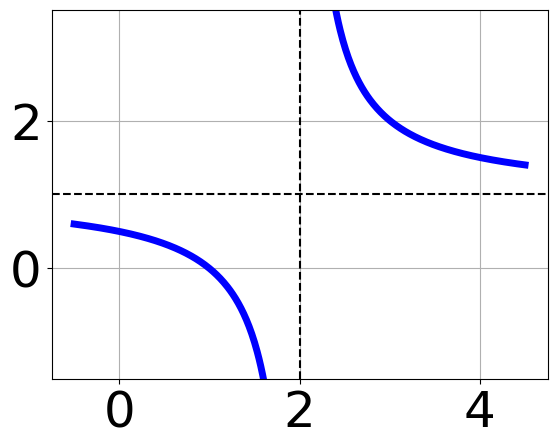
\includegraphics[width = 0.3\textwidth]{../Figures/rationalEquationToGraphCopyAC.png}\item 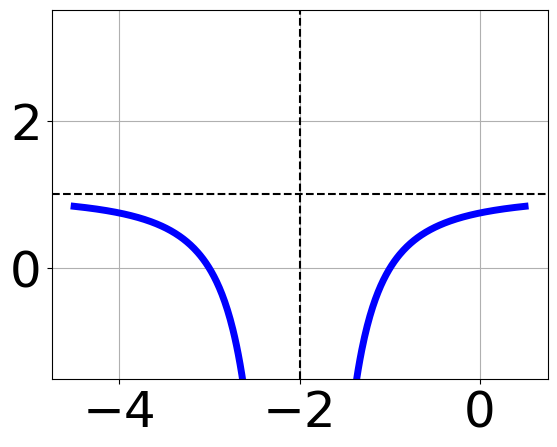
\includegraphics[width = 0.3\textwidth]{../Figures/rationalEquationToGraphCopyBC.png}\item 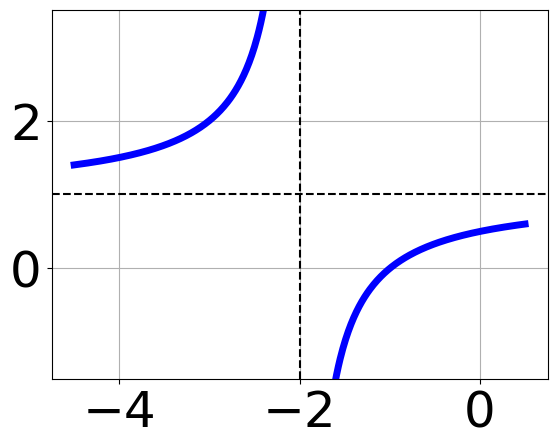
\includegraphics[width = 0.3\textwidth]{../Figures/rationalEquationToGraphCopyCC.png}\item 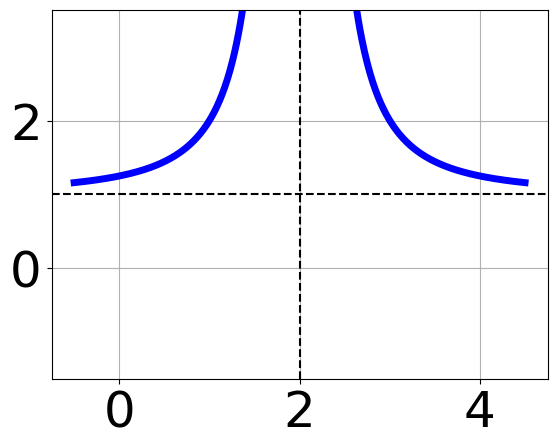
\includegraphics[width = 0.3\textwidth]{../Figures/rationalEquationToGraphCopyDC.png}\end{multicols}\item None of the above.
\end{enumerate} }
\litem{
Determine the domain of the function below.\[ f(x) = \frac{6}{15x^{2} -38 x + 24} \]\begin{enumerate}[label=\Alph*.]
\item \( \text{All Real numbers except } x = a, \text{ where } a \in [11.98, 12.15] \)
\item \( \text{All Real numbers.} \)
\item \( \text{All Real numbers except } x = a \text{ and } x = b, \text{ where } a \in [11.98, 12.15] \text{ and } b \in [29.98, 30.12] \)
\item \( \text{All Real numbers except } x = a, \text{ where } a \in [1.2, 1.24] \)
\item \( \text{All Real numbers except } x = a \text{ and } x = b, \text{ where } a \in [1.2, 1.24] \text{ and } b \in [1.31, 1.43] \)

\end{enumerate} }
\litem{
Solve the rational equation below. Then, choose the interval(s) that the solution(s) belongs to.\[ \frac{-8}{-5x + 2} + -9 = \frac{-9}{-45x + 18} \]\begin{enumerate}[label=\Alph*.]
\item \( x \in [-1.44,1.56] \)
\item \( x_1 \in [0.23, 0.43] \text{ and } x_2 \in [-0.44,3.56] \)
\item \( \text{All solutions lead to invalid or complex values in the equation.} \)
\item \( x \in [-0.37,-0.15] \)
\item \( x_1 \in [-0.37, -0.15] \text{ and } x_2 \in [-0.44,3.56] \)

\end{enumerate} }
\litem{
Choose the graph of the equation below.\[ f(x) = \frac{1}{x + 2} + 3 \]\begin{enumerate}[label=\Alph*.]
\begin{multicols}{2}\item 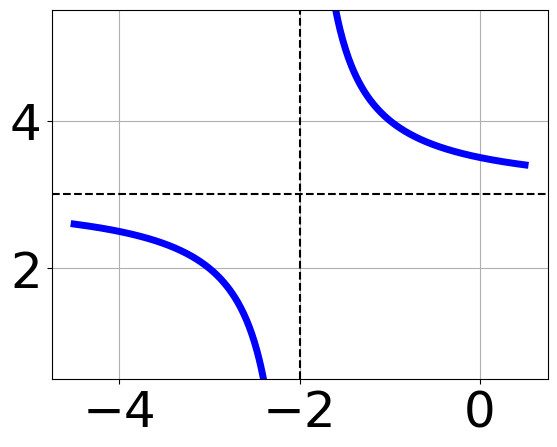
\includegraphics[width = 0.3\textwidth]{../Figures/rationalEquationToGraphAC.png}\item 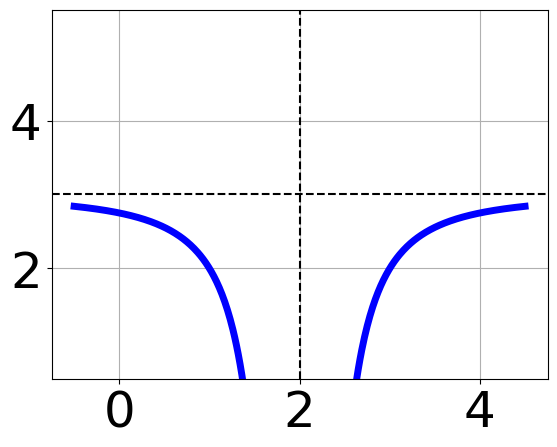
\includegraphics[width = 0.3\textwidth]{../Figures/rationalEquationToGraphBC.png}\item 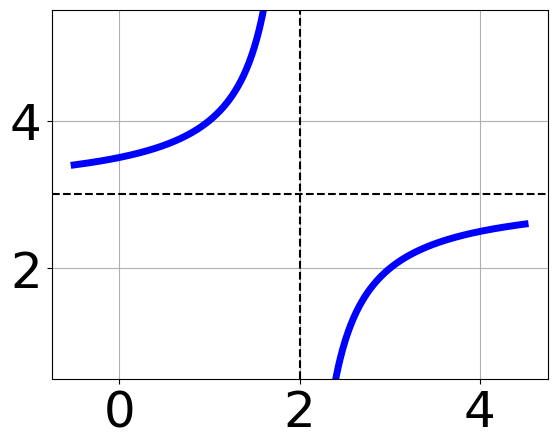
\includegraphics[width = 0.3\textwidth]{../Figures/rationalEquationToGraphCC.png}\item 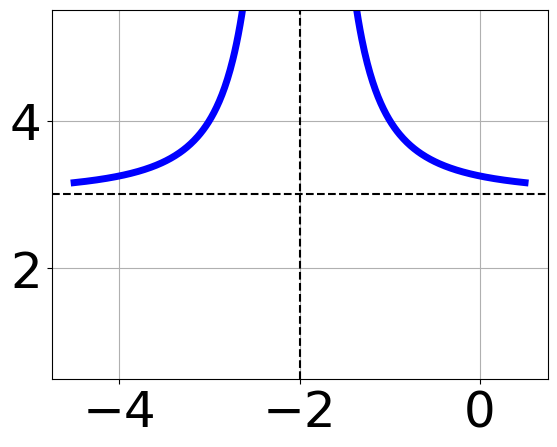
\includegraphics[width = 0.3\textwidth]{../Figures/rationalEquationToGraphDC.png}\end{multicols}\item None of the above.
\end{enumerate} }
\litem{
Choose the equation of the function graphed below.
\begin{center}
    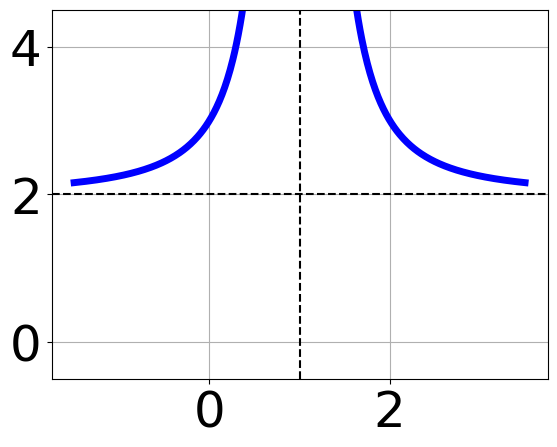
\includegraphics[width=0.5\textwidth]{../Figures/rationalGraphToEquationC.png}
\end{center}
\begin{enumerate}[label=\Alph*.]
\item \( f(x) = \frac{-1}{x - 1} + 0 \)
\item \( f(x) = \frac{1}{x + 1} + 0 \)
\item \( f(x) = \frac{-1}{(x - 1)^2} + 0 \)
\item \( f(x) = \frac{1}{(x + 1)^2} + 0 \)
\item \( \text{None of the above} \)

\end{enumerate} }
\litem{
Solve the rational equation below. Then, choose the interval(s) that the solution(s) belongs to.\[ \frac{-7x}{2x -7} + \frac{-7x^{2}}{10x^{2} -39 x + 14} = \frac{-4}{5x -2} \]\begin{enumerate}[label=\Alph*.]
\item \( x \in [-0.24,0.83] \)
\item \( \text{All solutions lead to invalid or complex values in the equation.} \)
\item \( x_1 \in [2.32, 5.4] \text{ and } x_2 \in [-0.04,0.83] \)
\item \( x_1 \in [0.7, 2.1] \text{ and } x_2 \in [-0.72,0.38] \)
\item \( x \in [2.32,5.4] \)

\end{enumerate} }
\litem{
Solve the rational equation below. Then, choose the interval(s) that the solution(s) belongs to.\[ \frac{-6x}{-5x + 4} + \frac{-4x^{2}}{-20x^{2} -4 x + 16} = \frac{-2}{4x + 4} \]\begin{enumerate}[label=\Alph*.]
\item \( x_1 \in [-0.08, 0.53] \text{ and } x_2 \in [-1.2,6.8] \)
\item \( x \in [-1.06,-0.81] \)
\item \( \text{All solutions lead to invalid or complex values in the equation.} \)
\item \( x \in [-1.47,-1.3] \)
\item \( x_1 \in [-0.08, 0.53] \text{ and } x_2 \in [-1.42,0.58] \)

\end{enumerate} }
\end{enumerate}

\end{document}